\documentclass[12pt]{article}
\usepackage[czech]{babel}
\usepackage[utf8]{inputenc}
\usepackage[plainpages=false,pdfpagelabels,unicode]{hyperref}
\usepackage[pdftex]{graphicx}
\usepackage[margin=3cm, includefoot]{geometry}

\begin{document}

\title{Zápočtové příklady z předmětu Matematické metody zpracování měření}
\author{Pavel Ondračka}
\maketitle

\section{Úloha 1}
\subsection{Zadání}
V tabulce (příloha 1) jsou hodnoty získané při 50-násobném opakování měření hodnoty x.

Odhadněte hledanou veličinu (použijte pokud možno větší počet metod). Pozor na případné vybočující hodnoty.

Testujte hypotézu o normálním (Gaussově) a dvojném exponenciálním (Laplaceově) rozdělení měřených dat.

\subsection{Test hypotézy o normálním rozdělení}
Normální rozdělení má tvar:
\begin{equation} f(x) = \frac{1}{\sqrt{2 \pi \sigma^2}} e^{-\frac{(x - \mu)^2}{2 \sigma^2}} \end{equation}
Pro normální rozdělení se střední hodnota určí jako aritmetický průměr, směrodatná odchylka jako $\sigma = \sqrt{\frac{1}{N}\sum_{i=1}^N(x_i - \bar{x})}$. 
Po dosazení experimentálních dat (příloha 1) vyjde: $\mu = \bar{x} = 1,7995$, $\sigma = 0,7659$.

Zběžnou prohlídkou vidíme že žádné měření není od střední hodnoty vzdáleno více jak $3\sigma$ a ve vzdálenosti $[2\sigma, 3\sigma]$ jsou celkem tři měření což je docela dobrá shoda (v těchto intervalech bychom při 50 měřeních očekávali dvě), tj. zdá se že soubor neobsahuje vybočující hodnoty.

\subsubsection{Pearsonův test}
Pro výpočet $\chi^2$ rozdělíme osu na $k$ intervalů, $n_i$ je počet hodnot na i-tém intervalu, $p_i$ je pravděpodobnost toho že měřená hodnota spadá do i-tého intervalu, $N$ je počet experimentálních hodnot. 

Platí:
\begin{equation}\chi^2 = \sum_{i=1}^k \frac{(n_i - Np_i)^2}{Np_i}\end{equation}

Pro výpočet je důležité, aby všechny intervaly měly přibližně stejné pravděpodobnosti. Při výpočtu bylo spočítáno 10 intervalů tak, že pro výše určené parametry $\mu$ a $\sigma$ má každý pravděpodobnost $p_i = 0,1$ (viz obrázek \ref{pearso1}).

\begin{figure}[h!]
  \centering
  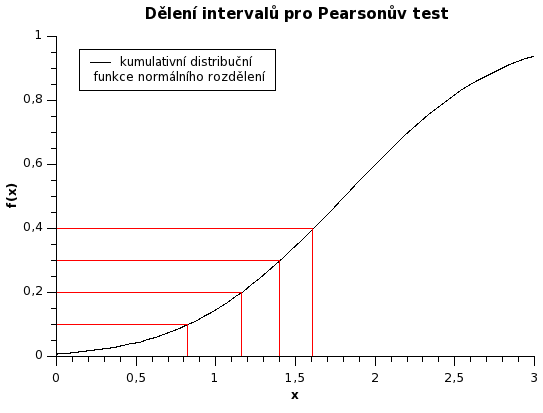
\includegraphics[width=13cm]{Graph5.png}
  \caption{Volba intervalů pro Pearsonův test (pouze několik prvních intervalů)}
  \label{pearso1} 
\end{figure}

\begin{table}[h!]
 \centering
 \begin{tabular}{|c|c|c|c|}
  \hline
  {\bf interval} & {\bf $n_i$} & {\bf $Np_i$}  & {\bf $\chi^2$}\\
   \hline \hline
	$(-\infty; 0,8177)$ & 4 & 5 & 0,2 \\
	$[0,8177; 1,1558)$ & 5 & 5 & 0 \\
	$[1,1558; 1,3980)$ & 6 & 5 & 0,2 \\
	$[1,3980; 1,6064)$ & 6 & 5 & 0,2 \\
	$[1,6064; 1,7994)$ & 5 & 5 & 0 \\
	$[1,7994; 1,9950)$ & 7 & 5 & 0,8 \\
	$[1,9950; 2,2012)$ & 4 & 5 & 0,2 \\
	$[2,2012; 2,4456)$ & 1 & 5 & 3,2 \\
	$[2,4456; 2,7835)$ & 6 & 5 & 0,2 \\
	$[2,7835; \infty)$ & 6 & 5 & 0,2 \\
	\hline
  \end{tabular}
  \caption{Výpočet $\chi^2$ pro normální rozdělení s parametry  $\mu = 1,7995$, $\sigma = 0,7659$}
  \label{intervaly}
\end{table}

Celková vypočítaná hodnota $\chi^2$ je $5,2$ (intervaly a výpočet jsou shrnuty v tabulce \ref{intervaly}). Pro zajímavost bylo spočítáno i $\chi^2$ pro intervaly $(-\infty, -3\sigma)$ , $[-3\sigma,-2\sigma)$,...,$[2\sigma,3\sigma)$,$[3\sigma, \infty)$. Pro toto dělení byl výsledek $\chi^2 = 1,2731$. Z toho je vidět, jak moc je volba intervalů při $\chi^2$ testu důležitá. Porovnáváním s tabulkami pro $\chi^2$ rozdělení vidíme, že hypotézu o normálním rozdělení nemůžeme vyloučit. Respektive můžeme ji vyloučit jen s pravděpodobností 10\%. 
\clearpage

\subsubsection{Kolmogorovův test}
Při Kolmogorovově testu porovnáváme kumulativní distribuční funkci $F(x)$ se skokovou empirickou funkcí $S_N(x)$ pro kterou platí

$$S_N = \left\{ \begin{array}{cl}
0 & \mathrm{pro }\,\, x<x_1 \\
i/N & \mathrm{pro }\,\, x \in [x_i, x_{i+1})\\
N & \mathrm{pro }\,\, x>=x_n \end{array}\right. $$

Průběh empirické a testované funkce je na obrázku \ref{fig:kol1}, odchylky jsou na obrázku \ref{fig:kol2}. Maximální odchylka $D_N$ má v našem případě hodnotu 0,0827 v bodě $x = 1,9487$. Testovaná veličina $\sqrt{N} D_N$ je 0,5848. Z tabulek vidíme, že $z_{0.89} = 0,580$. To znamená: můžeme zamítnout hypotézu o normálním rozdělení dat s rizikem 0,89.

\begin{figure}[h!]
  \centering
  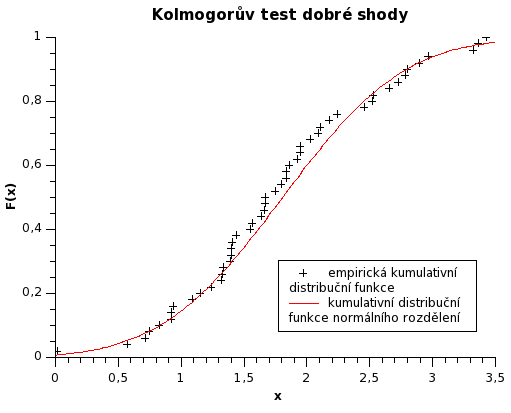
\includegraphics[width=13cm]{Graph2.png}
  \caption{Kolmogorovův test}
  \label{fig:kol1} 
\end{figure}

\begin{figure}[h!]
  \centering
  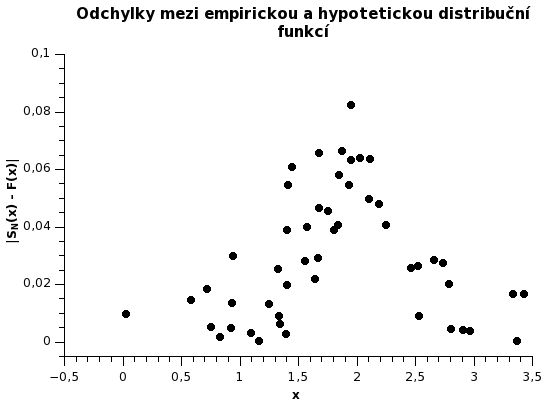
\includegraphics[width=13cm]{Graph6.png}
  \caption{Odchylky mezi $F(x)$ a $S_N(x)$}
  \label{fig:kol2} 
\end{figure}

\clearpage


\subsection{Test hypotézy o Laplaceově (dvojném exponenciálním) rozdělení}
Laplaceovo rozdělení má distribuční funkci ve tvaru:
\begin{equation}f(x)  = \frac{1}{2b} e^{-\frac{|x-\mu|}{b}}    \end{equation}
Kumulativní distribuční funkce má tvar:
\begin{equation}F(x)  = \frac{1}{2} [ 1 + \mathrm{sgn}(x-\mu) (1-e^{-\frac{|x-\mu|}{b}}) ] \end{equation}
Pro výpočet střední hodnoty $\mu$ se používá medián vzorku, disperze se pro toto rozdělení spočítá jako $2b^2$, kde nejpravděpodobnější hodnotu $b$ určíme jako: $b = \frac{1}{N}\sum_{i=1}^N|x_i - \mu|$. Dosazením testovaných dat zjistíme že $\mu = 1,7112$, $b = 0,6018$, disperze $D = 0,7243$ a $\sigma = 0,8510$. Se znalostí $\sigma$ můžeme nyní opět provést test na vybočující hodnoty, a je vidět že pouze jedna hodnota má od střední hodnoty vzdálenost větší jak $2\sigma$, což se zdá být v pořádku.

\subsubsection{Pearsonův test}
Stejně jako u normálního rozdělení bylo spočítáno deset intervalů se stejnou pravděpodobnostní hodnotou. Volbu intervalů a četnosti na jednotlivých intervalech shrnuje tabulka \ref{intervaly2}. Celková hodnota $\chi^2$ je stejná jako pro normální rozdělení: 5,2. Tj. opět nemůžeme hypotézu o Laplaceově rozdělení vyloučit.

\begin{table}[h!]
 \centering
 \begin{tabular}{|c|c|c|c|}
  \hline
  {\bf interval} & {\bf $n_i$} & {\bf $Np_i$}  & {\bf $\chi^2$}\\
   \hline \hline
	$(-\infty; 0,7417)$ & 3 & 5 & 0,8 \\
	$[0,7417; 1,1592)$ & 7 & 5 & 0,8 \\
	$[1,1558; 1,4024)$ & 7 & 5 & 0,8 \\
	$[1,4024; 1,5766)$ & 4 & 5 & 0,2 \\
	$[1,5766; 1,7112)$ & 4 & 5 & 0,2 \\
	$[1,7112; 1,8468)$ & 4 & 5 & 0,2 \\
	$[1,8468; 2,0180)$ & 4 & 5 & 0,2 \\
	$[2,0180; 2,2613)$ & 5 & 5 & 0 \\
	$[2,2613; 2,6787)$ & 4 & 5 & 0,2 \\
	$[2,6787; \infty)$ & 8 & 5 & 1,8 \\
	\hline
  \end{tabular}
  \caption{Výpočet $\chi^2$ pro Laplaceovo rozdělení s parametry  $\mu = 1,7112$, $b = 0,6018$}
  \label{intervaly2}
\end{table}

\subsubsection{Kolmogorovův test}
Kolmogorův test je na obrázku \ref{fig:kol3}. Maximální odchylka má hodnotu $D_n = 0,076$. Testovaná veličina $\sqrt{N}D_n$ má hodnotu 0,5374. Po nahlédnutí do tabulek vidíme, že hypotézu o Laplaceově rozdělení můžeme zamítnout s rizikem 94\%.

\begin{figure}[h!]
  \centering
  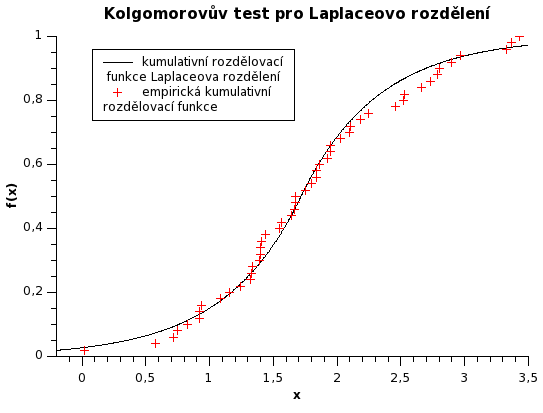
\includegraphics[width=13cm]{Graph7.png}
  \caption{Kolmogorovův test}
  \label{fig:kol3} 
\end{figure}





\section{Úloha 2}
\subsection{Zadání}
Odhadněte tři parametry $a,b,c$ závislosti $y=a \sin{x} + b \cos{x} +c$ proložením naměřených hodnot $x(i), y(i)$. Hodnoty $y(i)$ mají normální rozdělení se standardní odchylkou $dy(i)$.

\subsection{Výpočet}
Pro výpočet parametrů lineárního modelu hledáme minimum součtu čtverců odchylek hodnot naměřených a předpovězených modelem.
\begin{equation}S = \sum_{i=1}^N (y_i - f(x_i))^2 \frac{1}{(\mathrm{d}y_i)^2}\end{equation}
Konkrétně pro hledanou funkci:
\begin{equation}S = \sum_{i=1}^N (y_i - a\sin{x_i} - b\cos{x_i} - c)^2 \omega_i \,\,\,\mathrm{, kde}\,\,\, \omega_i = \frac{1}{(\mathrm{d}y_i)^2} \end{equation}
Z podmínky $\partial{S}/\partial{a}=\partial{S}/\partial{b}=\partial{S}/\partial{c}=0$ vyjde soustava tří rovnic:
\begin{equation}a\sum_{i=1}^N \sin^2{x_i} \omega_i + b \sum_{i=1}^N \sin{x_i}\cos{x_i} \omega_i + c\sum_{i=1}^N sin{x_i} \omega_i =  \sum_{i=1}^N y_i sin{x_i} \omega_i \end{equation}
\begin{equation}a\sum_{i=1}^N \sin{x_i}\cos{x_i} \omega_i + b \sum_{i=1}^N \cos^2{x_i}\omega_i + c\sum_{i=1}^N cos{x_i} \omega_i =  \sum_{i=1}^N y_i cos{x_i}\omega_i \end{equation}
\begin{equation}a\sum_{i=1}^N \sin{x_i} \omega_i + b \sum_{i=1}^N \cos{x_i}\omega_i + c\sum_{i=1}^N \omega_i =  \sum_{i=1}^N y_i \omega_i \end{equation}
Po dosazení experimentálních dat (příloha 2):
\begin{equation}\label{r1} 2672,24a + 460,21b + 1796,15c = 15722,08\end{equation}
\begin{equation}\label{r2}  460,21a + 3245,69b + 1061,54c = 7278,68\end{equation}
\begin{equation}\label{r3} 1796,15a + 1061,54b + 5917,93c = 34377,15\end{equation}
Hledané parametry jsou tedy: $a=2,470\,\,\, b=0,252\,\,\, c=5,014$
Koeficienty v rovnicích (\ref{r1}),(\ref{r2}) a (\ref{r3}) jsou zároveň prvky Hesiánu $\hat{H}$. Z něj můžeme určit kovariantní matici $\hat{C}$.

$$
\hat{C} = \hat{H}^{-1} = \left(\begin{array}{ccc}
\sigma_a^2 & \sigma_a\sigma_b & \sigma_a\sigma_c \\
\sigma_a\sigma_b & \sigma_b^2 & \sigma_b\sigma_c \\
\sigma_a\sigma_c & \sigma_b\sigma_c & \sigma_c^2 \end{array}\right)
$$

$$\hat{C}=
\left(\begin{array}{ccc}
2672,24 & 460,21 & 1796,15\\
460,21 & 3245,69 & 1061,54\\
1796,15 & 1061,54 & 5917,93
\end{array}\right)^{-1} = $$


$$\left(\begin{array}{ccc}
 0,0004715 & -0,0000213 & -0,0001392\\
-0,0000213 & 0,0003282 & -0,0000524\\
-0,0001392 & -0,0000524 & 0,0002206\end{array}\right)$$
Směrodatné odchylky jsou tedy $\sigma_a = 0,022\,\,\, \sigma_a = 0,018\,\,\,\sigma_c = 0,015$.

Úpravou kovariantní matice tak, abychom na hlavní diagonále dostali jedničky, vzniká korelační matice $\hat{D}$.

$$\hat{D} = \left(\begin{array}{ccc}
 1 & -0,0452 & -0,2952\\
-0,0649 & 1 & -0,1597\\
-0,6310 & -0,2375 & 1\end{array}\right)$$





Pro zajímavost porovnejme lineární model s jiným fitovacím algoritmem, konkrétně škálovaným Levenberg-Marquartovým algoritmem (1000 iterací, tolerance 0,0001, uniformní výchozí parametry a=1, b=1, c=1). Na obrázku \ref{fig:h} můžeme vidět že navzdory velmi výraznému rozdílu ve složitosti, jsou výsledky velmi podobné. Tabulka \ref{ref:tab}

\begin{table}[h!]
 \centering
 \begin{tabular}{|c|c|c|}
  \hline
  {\bf } & {\bf lineární model} & {\bf Levenberg-Marquardt} \\
   \hline \hline
	$a \pm \sigma_a $ & $2,470 \pm 0,022$ & $2,465 \pm 0,033$ \\
	$b \pm \sigma_b $ & $0,252 \pm 0,018$ & $0,219 \pm 0,027$ \\
	$c \pm \sigma_c $ & $5,014 \pm 0,015$ & $4,990 \pm 0,023$ \\
	\hline
  \end{tabular}
  \caption{Porovnání parametrů}
  \label{ref:tab}
\end{table}


\begin{figure}[h!]
  \centering
  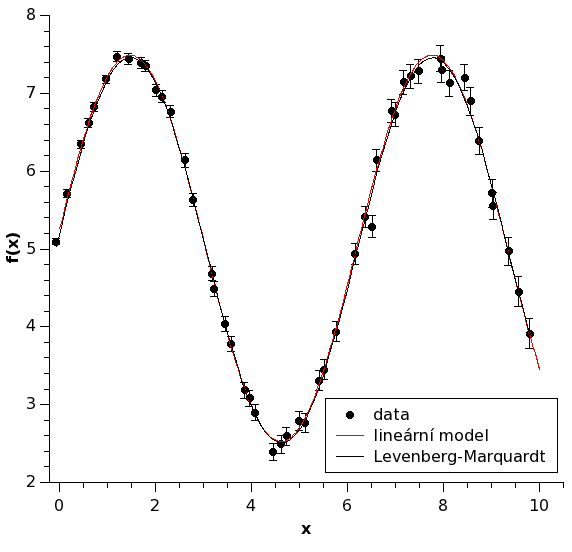
\includegraphics[width=13cm]{Graph1.png}
  \caption{Porovnání shody lineárního a Levenberg-Marquartova modelu s experimentálními daty}
  \label{fig:h} 
\end{figure}
\clearpage

\appendix
\section{Přílohy}
\subsection{Data pro úlohu 1}
\begin{verbatim}
1	1,3915
2	0,9369
3	1,2426
4	1,3383
5	2,1075
6	2,6577
7	0,5742
8	1,4394
9	2,0247
10	0,7172
11	0,8263
12	1,6655
13	1,7501
14	1,9476
15	2,9652
16	2,8985
17	1,9255
18	3,4267	
19	1,9487
20	2,4604
21	1,3288
22	1,5652
23	3,3277
24	2,2438
25	0,9192
26	1,4096
27	2,1835
28	3,3655
29	0,0189
30	1,8360
31	1,8012
32	1,3981
33	1,6722
34	1,1569
35	1,0887
36	2,5276
37	1,5489
38	0,9235
39	0,7511
40	2,7289
41	1,3995
42	1,8413
43	1,6704
44	2,5197
45	1,3197
46	1,6405
47	2,8026
48	1,8637
49	2,7831
50	2,0945
\end{verbatim}

\subsection{Data pro úlohu 2}
\begin{verbatim}
xi	      yi       dyi
-0,0696   5,1000   0,0422
0,1630   5,7179   0,0510
0,6085   6,6251   0,0583
0,4539   6,3503   0,0555
0,7176   6,8277   0,0551
0,9664   7,1846   0,0571
1,1958   7,4789   0,0657
1,4430   7,4432   0,0694
1,6962   7,3975   0,0669
1,7911   7,3544   0,0681
2,0141   7,0446   0,0760
2,1367   6,9638   0,0743
2,3148   6,7712   0,0818
2,6169   6,1457   0,0884
2,7811   5,6325   0,0826
3,1762   4,6884   0,0931
3,2203   4,4918   0,0947
3,4483   4,0455   0,0948
3,5700   3,7806   0,0956
3,8491   3,1892   0,1065
3,9626   3,0891   0,1020
4,0745   2,9052   0,1055
4,4485   2,3929   0,1099
4,6186   2,4949   0,1100
4,7327   2,6027   0,1163
4,9929   2,7937   0,1199
5,1176   2,7715   0,1259
5,4021   3,3151   0,1259
5,5104   3,4581   0,1241
5,7613   3,9459   0,1316
6,1499   4,9426   0,1328
6,3611   5,4142   0,1374
6,5127   5,2921   0,1421
6,6023   6,1462   0,1428
6,9170   6,7773   0,1446
6,9851   6,7343   0,1511
7,3081   7,2273   0,1533
7,1596   7,1466   0,1538
7,4771   7,2878   0,1595
7,9567   7,3113   0,1654
7,9360   7,4479   0,1669
8,1198   7,1330   0,1713
8,4318   7,2068   0,1667
8,5624   6,9019   0,1761
8,7380   6,3930   0,1742
9,0072   5,7218   0,1772
9,0282   5,5603   0,1779
9,3477   4,9771   0,1808
9,5572   4,4602   0,1868
9,7904   3,9186   0,1943
\end{verbatim}
\end{document}
